\subsection{Setup}
In the experiments we process all the text data into lower case and use the BERT models "bert-base-uncased" and "bert-large-uncased". We implemented all experiments using the transformers library \citep{wolf2019huggingfaces}.

To compute the rotation matrices by DensRay, we need a gendered word list as label, and some corpus. For the word list, we get 23 masculine words and 23 feminine words from the "family" category\footnote{http://download.tensorflow.org/data/questions-words.txt} of the Google analogy test set \citep{mikolov2013efficient}, and label them as 1 and -1. As the input corpus, we collect text data from Wikipedia that contains 5,000 (10,000) occurrences of words in the gendered list for BERT base (large) model. We carefully balance the occurrences such that the number of male and female samples are equal. We set  $\alpha_{\neq}=\alpha_{=}=0.5$, as we have balanced the training samples from the corpus.

As to compare with prior works, we compared with the post-processing method proposed by \citet{mu2018all} to eliminate gender bias as \citet{karve2019conceptor} introduced. 

\subsection{Results on OCCTMP}
Results about our experiments on OCCTMP are summarized in \tabref{t:templates1}. Two OCCTMP examples are given in \tabref{t:templates2}. It shows that DensRay can mitigate the gender bias in BERT: the average difference between predicting he/she drops to around two third (e.g., bert-base from 0.47 to 0.11).
\begin{table}[ht]
\centering
\footnotesize
\begin{tabular}{lcccc}
\hline
model & prob(he) & prob(she) & diff & var\\
\hline
bert-base & 0.66 & 0.19 & 0.47 &0.16\\
bert-base-Mu & 0.35 & 0.42 & -0.07  &0.03\\
bert-base-densray & 0.48 & 0.37 & {0.11} &0.02\\
\hline
bert-large  & 0.63 & 0.19 & 0.44  &0.13\\
bert-large-Mu & 0.40 & 0.23 & 0.17  &0.02\\
bert-large-densray  & 0.47 & 0.31 & {0.16} &0.02 \\
\hline
\end{tabular}
\caption{\tablabel{t:templates1}
BERT debiasing results on OCCTMP. \textit{bert-base} and \textit{bert-large} are the original model without debiasing. \textit{prob(he)} is the average probability that model predict \textit{he} as the [MASK] in OCCTMP. \textit{var} is the variance of the differences between the probability of BERT predicts [MASK] as \textit{he} and \textit{she}.} 
\end{table}
\begin{table}[ht]
\centering
\footnotesize
\begin{tabular}{llcc}
\hline
sentence & model & prob(he) & prob(she)\\
\hline
[MASK] is a & 
\scriptsize bert-base 
& 0.72 & 0.19\\
adjunct professor. & 
\scriptsize bert-base-densray 
& 0.44 & 0.47\\
&\scriptsize bert-large
& 0.72 & 0.22\\
&\scriptsize bert-large-densray& 0.40 & 0.53\\
\hline
[MASK] is a 
&\scriptsize bert-base 
& 0.63 & 0.23\\
administrator.  
&\scriptsize bert-base-densray 
& 0.50 & 0.38\\
&\scriptsize bert-large & 0.65 & 0.23\\
&\scriptsize bert-large-densray & 0.45 & 0.37\\
\hline
\end{tabular}
\caption{\tablabel{t:templates2}
OCCTMP examples with prediction probabilities.}
\end{table}
\subsection{Results on WEAT}
In WEAT we measure the effect size $d$-value and the oneside $p$-value of the permutation test. For the $d$-value, the closer to zero, the less gender bias.  We also prefer a high $p$-value (at least 0.05) to accept the null hypothesis which indicates the lack of gender bias. Follow the same WEAT word lists setup as \citet{karve2019conceptor}, the results on WEAT is shown on \tabref{t:weat1}.
\begin{table}[ht]
\centering
\scriptsize
\begin{tabular}{clcccc}
\hline
&&\multicolumn{2}{c}{WEAT}&\multicolumn{2}{c}{SEAT}\\
\hline
category & model & d & p& d & p\\
\hline
C6 & bert-base & 0.66 & 0.08 &0.11&0.25\\
& bert-base-Mu & 0.15 & 0.38&0.48&0.10\\
&bert-base-densray & 0.62 & 0.12&-0.11&0.75\\
%& bert-large & 1.57 & $0.00^{*}$ \\
%&bert-large-Mu & 0.80 & 0.06 \\
%& bert-large-densray & 0.76 & 0.07\\
\hline
C7 & bert-base & 0.60 & 0.11 &0.72&0.01\\
& bert-base-densray & -0.07 & 0.56&-0.09&0.72\\
& bert-base-densray & 0.09 & 0.45&-0.11&0.26\\
%& bert-large & -0.40 & 0.75 \\
%& bert-large-Mu & -0.51 & 0.83\\
%& bert-large-densray & -0.06 & 0.45\\
\hline
C8& bert-base & 0.78 & 0.08 &1.00&0.01\\
& bert-base-Mu & -0.29 & 0.68&0.36&0.03\\
& bert-base-densray & 0.03 & 0.47&0.75&0.01\\
%& bert-large & -0.60 & 0.87  \\
%& bert-large-Mu & 0.78 & 0.06\\
%& bert-large-densray & 0.20 & 0.33\\

\hline
\end{tabular}
\caption{\tablabel{t:weat1}
BERT debiasing results on WEAT. * shows significant gender bias.}
\end{table}
\subsection{Impact on Model Performance}
It is crucial that debiasing methods do not harm downstream performance of BERT models.Thus we test the perplexity of language modeling on the Wikitext-2 \citep{merity2016pointer}, a subset of Wikipedia with 2 million words. We also test on some GLUE tasks \citep{wang2018glue}. For all the tests we follow the same setup as \citet{wolf2019huggingfaces}\footnote{https://huggingface.co/transformers/}. \tabref{t:glue1} shows that DensRay debiasing gets comparable results with the original models on Wikitext-2 and GLUE tasks.
\begin{table*}[ht]
\centering
\footnotesize
\begin{tabular}{lcccccccccc}
\hline
model & Wikitext-2&CoLA &SST-2&MRPC&STS-B&RTE&WNLI\\
\hline
bert-base &3.77&49.15&92.09&85.86&82.66&62.82&52.11\\
bert-base-mu &3.95&45.53&91.74&82.48&82.60&63.54&56.34\\
bert-base-densray &3.81&48.04&91.74&84.89&82.43&63.90&53.52\\
\hline
bert-large &3.29& 47.93&94.90&89.30&87.60&70.10&65.10\\
bert-large-Mu &3.85& 47.45&93.95&85.01&82.33&67.12&63.02\\
bert-large-densray &3.35& 48.91&94.02&88.84&85.63&67.78&64.48\\
\hline
\end{tabular}
\caption{\tablabel{t:glue1}
Language modelling perplexity and GLUE tasks performance.}
\end{table*}
\subsection{Discussions}
\subsubsection{Compare DensRay and Hard Debiasing}
Here we compare the difference between DensRay and the HArd debiasing by \citep{mu2018all}. With their objectives, we can find that DensRay will produce meaningful direction on the gender axis, then male bias and female bias are distributed on different sides of the axis. While Hard debiasing does not necessarily produce such a direction, their direction is provided by the embedding model.
\begin{figure}[h]
	\centering
	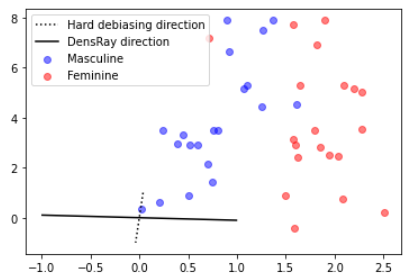
\includegraphics[width=0.9\linewidth]{example.png}
	\caption{Gender direction on gendered words.}
	\figlabel{fig:example}
\end{figure}
\subsubsection{Debiasing on Attention Heads}
Here we applied DensRay on the attention heads in BERT to debias on OCCTMP, the heatmap \figref{fig:heads} shows that the debiasing effect of one single attention head is not obvious, with diff scores all around 0.4 - 0.5. Due to the lack of dimensions and the distribution of gender features in the attention heads, we chose to apply DensRay on layers as debiasing method.
\begin{figure}[h]
	\centering
	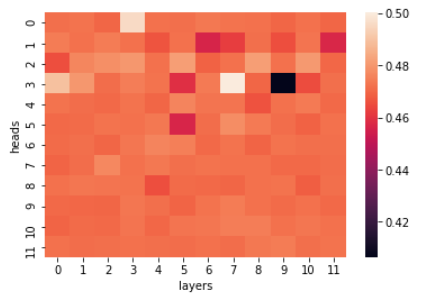
\includegraphics[width=0.9\linewidth]{heatmap_heads}
	\caption{DensRay debiasing on each single attention head in BERT base, measured by \text{diff} on OCCTMP.}
	\figlabel{fig:heads}
\end{figure}


\subsubsection{Number of Training Samples}
In the experiments, we regarded the occurrences of the same word in the corpus as independent words with the same gender label, as a data augmentation appraoch. We also and used balanced samples for masculine and feminine words. Now we analyze the impact of these processes.
DensRay is essentially a supervised learning method. In the case of insufficient labels, it is difficult for supervised learning to extract useful features. Treating different occurrences as different words greatly enriches training samples. As shown in figure, the debiasing results improve with an increased number of training samples.

The same as other projection-based debiasing methods \citep{bolukbasi2016man,zhao2019gender,dev2019attenuating, karve2019conceptor}, the premise of DensRay debiasing is that the bias direction should be correct. If the sample is unbalanced, the bias direction computed by DensRay will be biased towards either the male or the female, resulting in deleting the gender subspace during debiasing will reverse the gender bias (e.g. there are more masculine words in unbalanced text data, thus the embeddings will be biased towards female after biased). The figure also shows that balanced training sample improved the debiasing performers. 
\begin{figure}[ht]
    \centering
    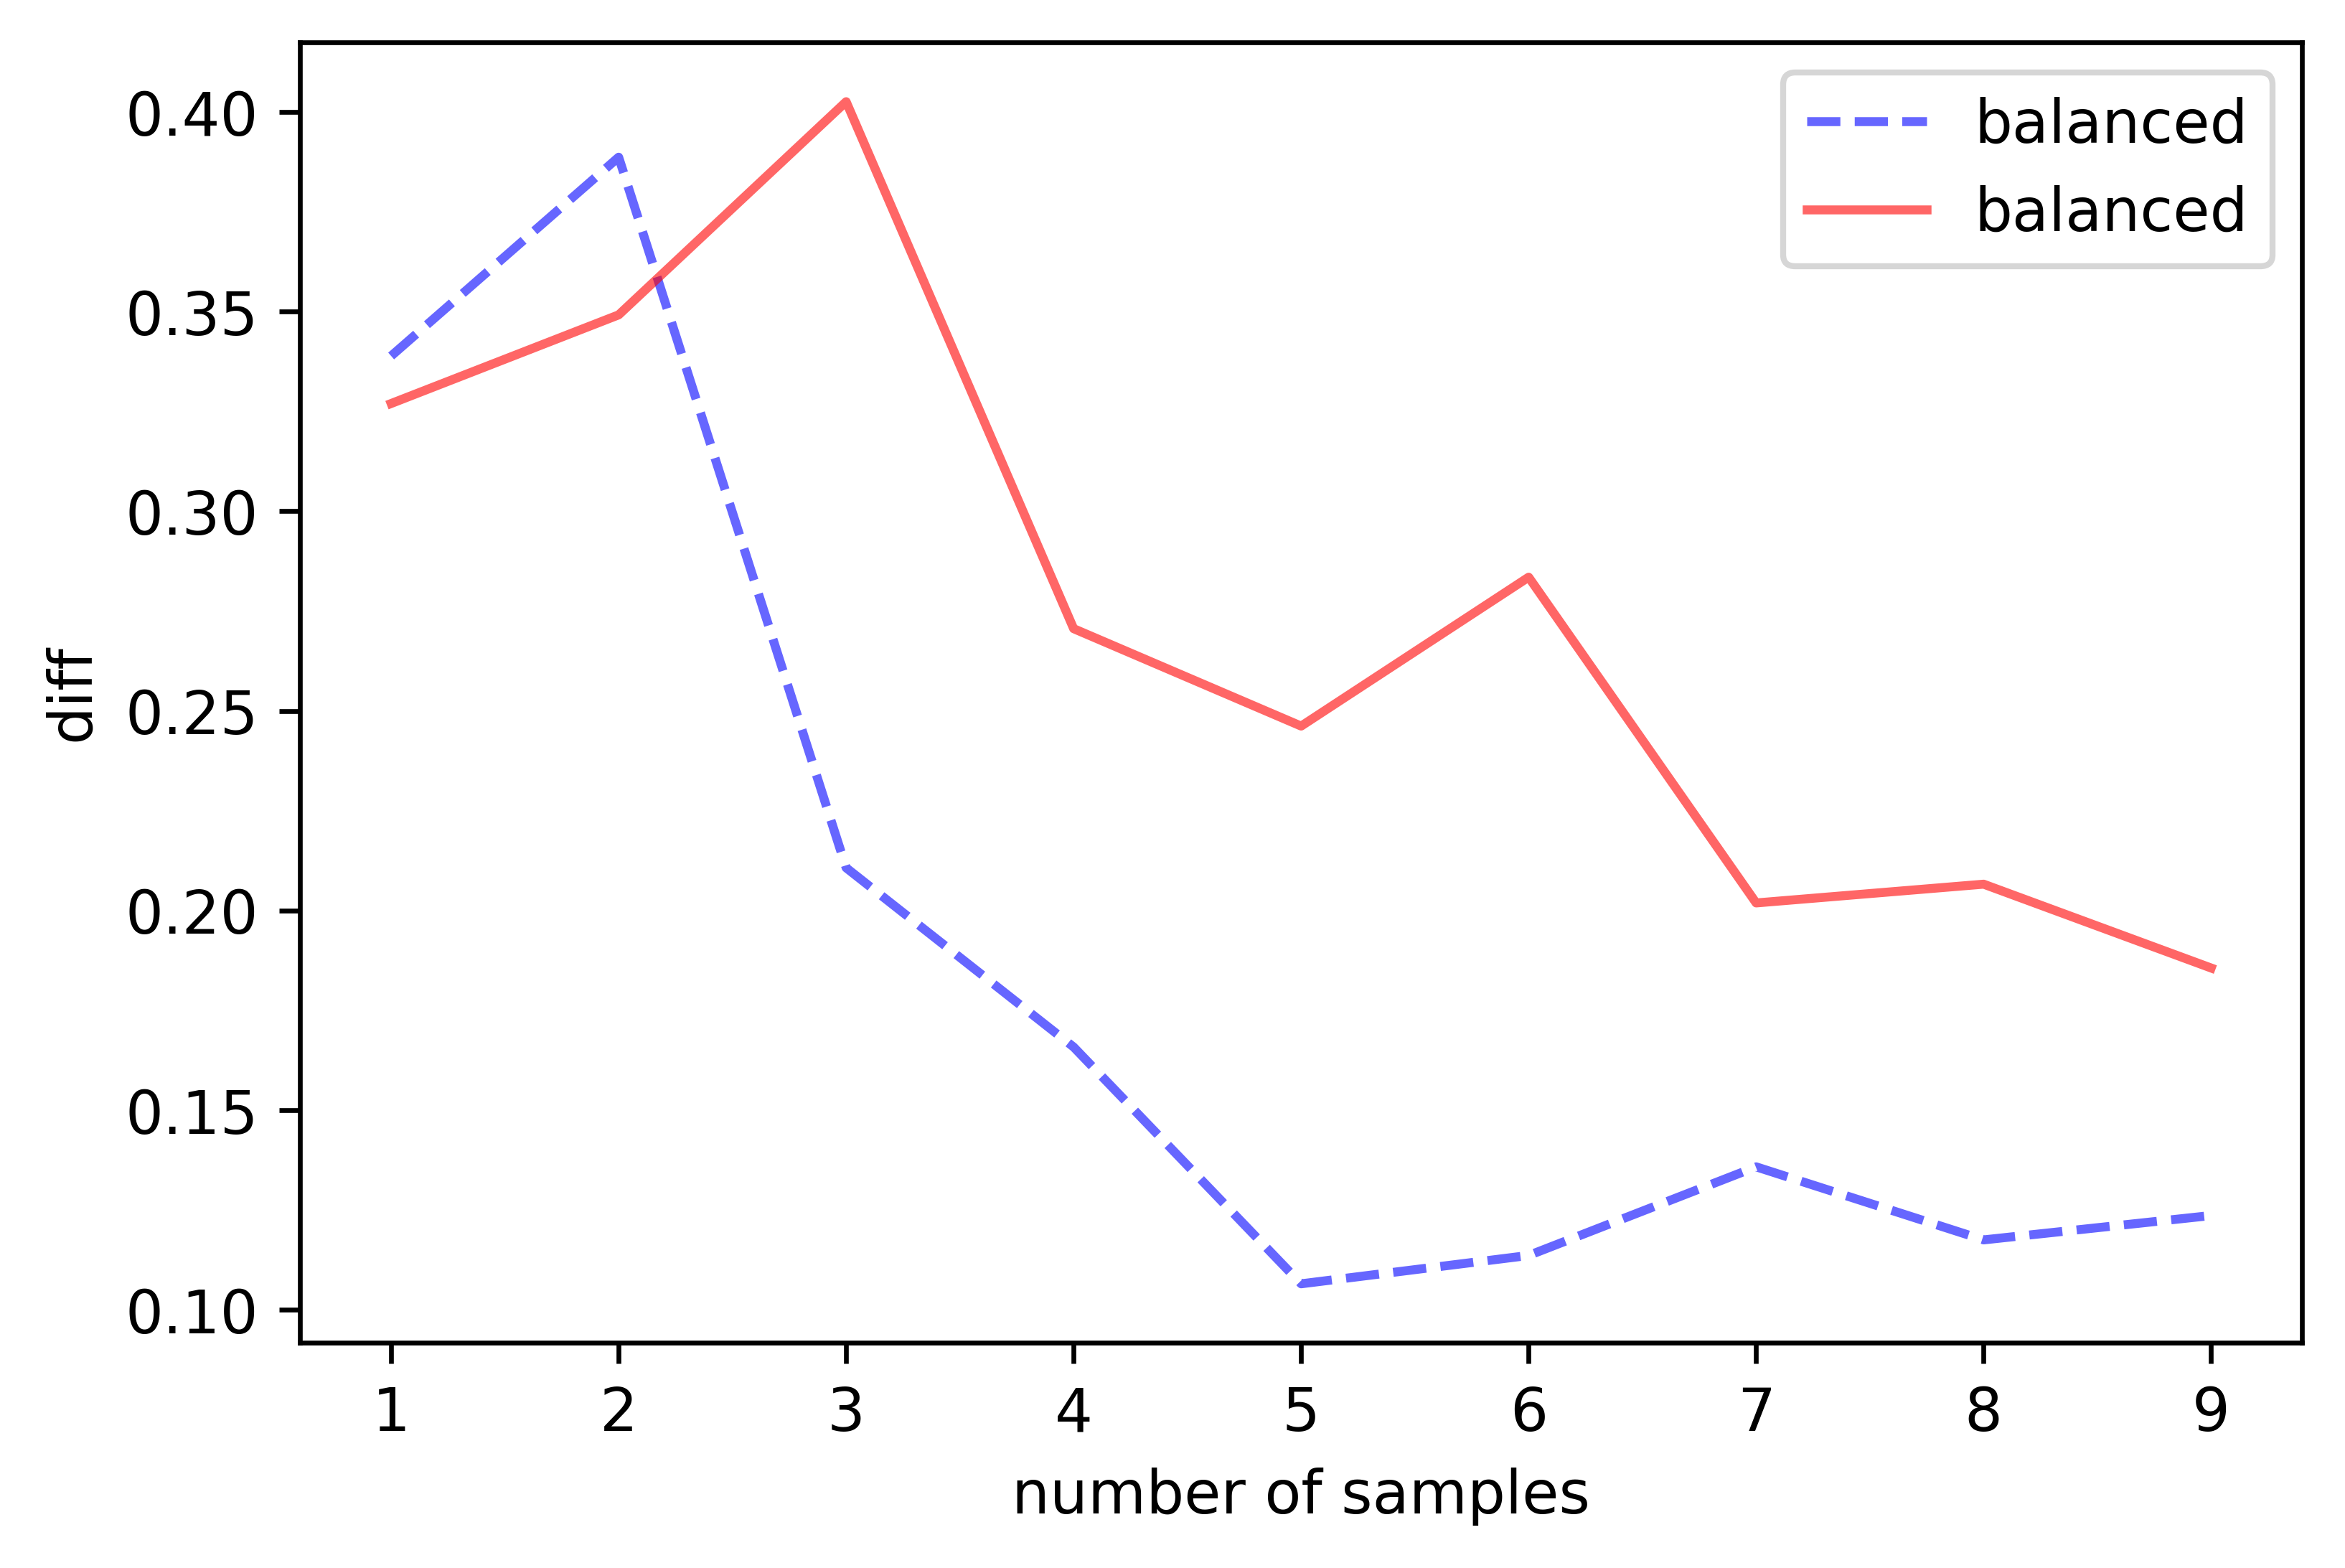
\includegraphics[width=6cm,height=3cm]{samples}
    \caption{DensRay debiasing results on OCCTMP with different number of samples.}
    \label{fig:my_label}
\end{figure}

\subsubsection{Balancing Gender Bias}
In this experiment, we used the method of removing the first dimension (replacing its value by $0$) of the gender interpreteble subspace to remove gender bias. Here we explore some other ways.

We explored three other ways to remove bias: 1) replace the first dimension of the gender interpreteble subspace with the mean value of the first dimension of the training samples. 2) standardize the first dimension. 3) replace the first dimension with a small random variable sampled from Gaussian distribution. All of them did not perform well. We further checked the mean and found that the mean of the different layers is not stable around 0, which is a problem worthy for further exploring. We also tried to delete more dimensions. However removing more dimensions does not improve the debiasing results significantly, while harming the model performance significantly.


\subsubsection{Debiasing on different BERT layers}
Here we only apply DesnRay on one BERT layer at a time. See \figref{fig:layersbase} to illustrate the results of layers on our templates and the three WEAT categories. It shows that the debiasing effect on the 7-10 layer is more visible than on the other layers in BERT base model.
\begin{figure}[ht]
	\centering
	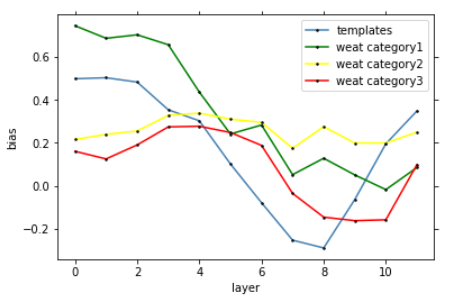
\includegraphics[width=0.9\linewidth]{layers_base}
	\caption{Debiasing on each single layer on BERT base. Bias is measured by \text{diff} on the templates and $d$-value on WEAT categories.}
	\figlabel{fig:layersbase}
\end{figure}

